
%==========================================================
\section{Introduction}
  Water scarcity is the lack of sufficient available water resources to meet water needs within a region. It affects every continent and around 2.8 billion people around the world at least one month out of every year. More than 1.2 billion people lack access to clean drinking water\cite{wikiwaterscarcity}.

  Till now, there are lots of researches about this topic.\cite{research1}\cite{research2}\cite{research3}. However, these researches mainly concern about the statistics in this problem, little dynamics were found. To do predictions, dynamics must be taken into consideration. In this paper, we investigate the internal mechanism among possible relevant quantities, and used this mechanism to obtain proper predictions about future water usability. Further more, we introduce some intervention plans to improve the water availability.
\section{Nomenclatures}

\begin{table}[!htb]

  \centering
  \begin{tabular}{||l|c||}
    \hline
    $P$/10k people   & Population \\
    \hline
    $\text{GDP/100m CNY}$ & Gross Domestic Product \\
    \hline
    $\text{PCGDP/ CNY per person}$ & Per Capita Gross Domestic Product \\
    \hline
    $\text{CAP/100m CNY}$ & Cross Agricultural Product \\
    \hline
    $\text{AWC/100m}\text{ m}^3$ & Agricultural Water Consumption per year \\
    \hline
    $\text{IWC/100m}\text{ m}^3$ & Industrial Water Consumption per year \\
    \hline
    $\text{DWC/100m}\text{ m}^3$ & Domestic Water Consumption per year \\
    \hline
    $\text{TWR/100m}\text{ m}^3$ & Total Water Resource \\
    \hline
    $\text{SWR/100m}\text{ m}^3$ & total Surface Water Resource \\
    \hline
    $\text{UWR/100m}\text{ m}^3$ & total Underground Water Resource \\
    \hline
    $\text{PCGDP/CNY}$ & Per Capita Gross Domestic Product \\
    \hline
    $\text{IA/kha}$ & Irrigation Area \\
    \hline
    $\text{ISP/10k ton}$ & Iron and Steel Production \\
    \hline
    $\text{ElP/100m kWh}$ & Electricity Production. \\
    \hline
    $\text{EnC/percentage}$ & Engel's Coefficient \\
    \hline
    $A/\text{m}^3 \text{per person}$          & Annual water supplies per person \\
    \hline
  \end{tabular}
  \caption{Nomenclatures System}
  \label{tab: Nomenclatures sys}
\end{table}

\section{Model of water supply ability}
  When it come to the water supply ability of a region, a country or even the world. We often use the measurement called annual water supplies per person($A$) for description\cite{AbilityMeasure}. We can set three levels to classify the ability of several regions (Table~\ref{tab: water supply ability}).

  \begin{equation}
  A = \left(\sum{\text{WaterConsumption}}\right)/\text{Population}
  \label{equ: Ability}
  \end{equation}


  \begin{table}[!htb]
    \centering
    \begin{tabular}{|c||c|c|}
    \hline
    level 1   & $A>1700$ & Sufficient \\
    \hline
    level 2   & $1700>A>1000$ & stressful \\
    \hline
    level 3   & $1000>A$ & scarce \\
    \hline
    \end{tabular}
    \caption{water supply ability}
    \label{tab: water supply ability}
  \end{table}

To cover the internal dynamics of the water flow and the water storage change, we introduce following model.

  \subsection{Model Introduction}
    Water circulation is a rather complicated process, which make it almost impossible for us to design a purely fundamental model to include all the variables and their relations. Nevertheless, if we just collect all the data and using fitting method as our predicting model, it will be too trivial and old-fashioned. To solve this paradox, we introduce a phenomenological model which is quite normal in particle physics and other related field. Our model includes two main parts:
    \begin{itemize}
      \item prominent external parameters: a several statistical parameters about a region like population, GDP and so on.
      \item internal dynamic variables: find out the relation between prominent external parameters and internal variables including Agriculture Water Consumption, Industrial Water Consumption and Domestic Water consumption.
    \end{itemize}
    The prominent external parameters comes from the statistic numbers and it's fitness, while the internal dynamics variables is mainly based on prominent parameters, which makes them indirectly depend on time in our model.

  \subsection{Model Hypothesis}
    Our model is based on following hypothesis:

    \begin{enumerate}[\textbf{Hypothesis} 1]
      \item We presume that the total water usage can be divided into three parts: Industrial, Agricultural and Domestic. And the main purpose of this model is to investigate these 3 quantities and relevant quantities. This hypothesis is plausible because the remaining fractions are relatively so small.
      \item Because that the water supply is one of the supporting industry in human society, we presume the water supply can always adjust itself to meet the need of the demand to a very large extent annually. Thus, each part of the water usage is treated as the function of more prominent parameters such as populations, PCGDP, irrigation area and so on.
      \item We presume that the prominent parameters mentioned above can specify the development information of human society. That is to say they are only the function of time itself. This hypothesis is plausible because in relatively short time period, say 15 years for example, the evolution of such fundamental quantities is determined by the intrinsic property of the society, but have little relationship with the water usage we interested in.
      \item We use specific model to fit the prominent parameters, and presume that the model will be legitimate in the following 15 years. This hypothesis is plausible because that the model we choose to fit is proper and the data is plentiful.
      \item According to the above description, each part of the water usage is treated as the function of prominent parameters. We further presume that they act linearly on corresponding water usage. This hypothesis is plausible for mainly 2 reasons. Firstly, we will find in later discussion that all values taken into consideration change slowly with respect of time. So from the Taylor series viewpoint, the complex interactions exist in the system can be finely interpolated using a linear interacting model.  Secondly, we intendedly choose the prominent parameters that can independently describe one aspect of the given society. So the interaction between these quantities are designed to be ignorable.
    \end{enumerate}

  \subsection{Model Structure}

    \begin{figure}[!h]
    \centering
    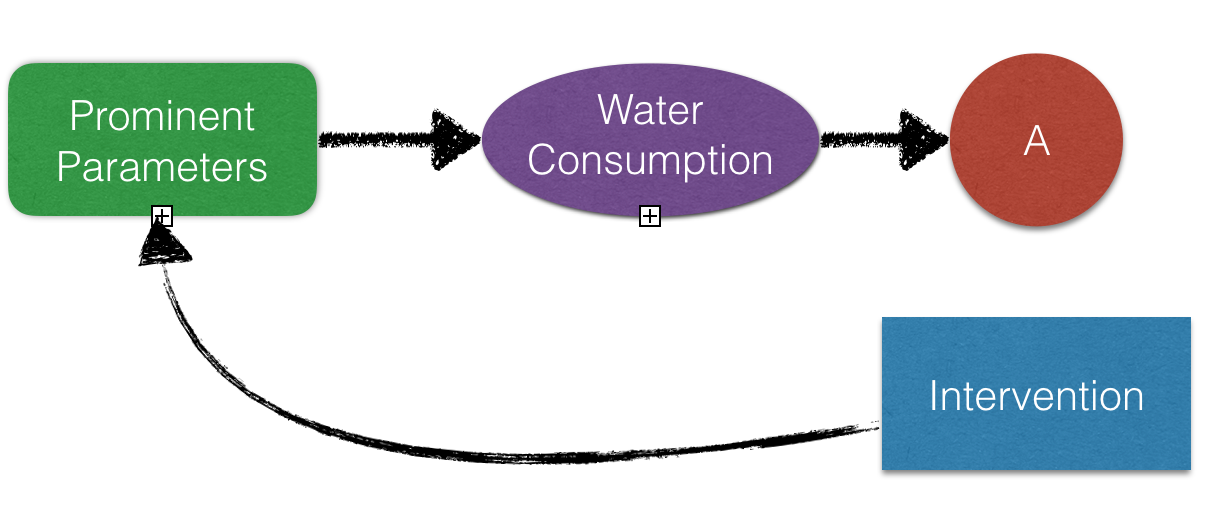
\includegraphics[width = 0.9\textwidth]{picture/struct.png}
    \caption{structure}
    \label{fig: structure}
    \end{figure}
    Our model's structure is pretty clear.
    We using some prominent external parameters as the input of our dynamic system. To determine the water supply ability of a region, the most important part is the water flow which means the total amount of industrial, agricultural and residential consumption. The season we can use the consumption to measure the supply it that they must be the same during a long period just like the electricity use equal to the electricity produce.

    $$
    \langle \text{Consumption}\rangle = \langle \text{Supply} \rangle
    $$

    The $W$ and $\bar{W}$ is a crucial conception in our dynamic part, $W$ stand for the total clean water resource over a period, while the $\bar{W}$ is the total wasted water resource which can be transfered into $W$ after several processing steps.

  \subsection{Model Prominent Parameters}

    The prominent parameters are some thing the dynamics part heavily rely on, to find the prominent parameters, we need to investigate the relation between some alternative parameters and consumptions according to the past data. In other words, prominent parameters are not given before a specific research object is given, we just give some alternative parameters and using the past data to determine which is better related and which is less related to our dynamic part variables.

    Generally, there are several important alternative parameters like: Population, GDP Per Capita are of course important statistic numbers. Moreover, Agricultural Irrigation Area play an important role in agricultural consumption, Iron and Steel Production is also important in industrial consumption, and Engel's coefficient is an important statistical number about residential living which make it important in residential consumption.

  \subsection{Model Dynamics}

    \begin{wrapfigure}{l}{0.35\textwidth}
    %\begin{center}
    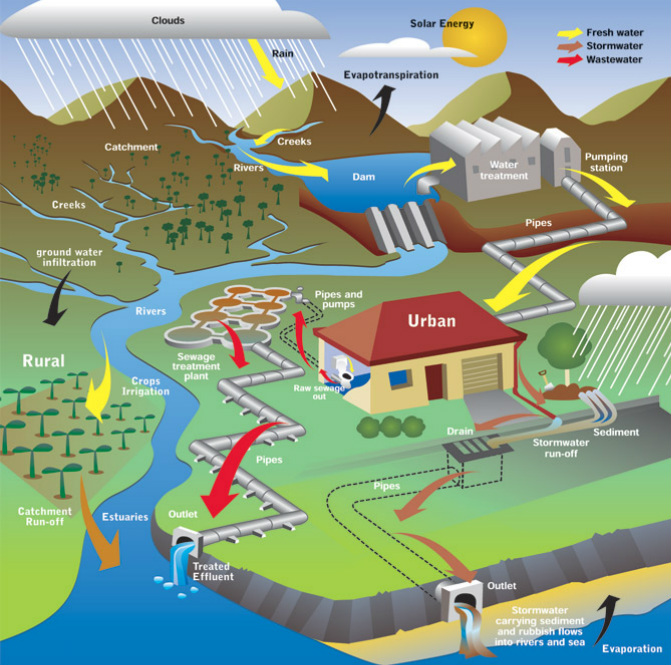
\includegraphics[width = 0.35\textwidth]{picture/UrbanWaterCycle.jpg}
    \caption{water cycle\cite{WaterCycle}}
    \label{water cycle}
    %\end{center}
    \end{wrapfigure}
    The dynamics part of our model is inspired by the water cycle(Figure~\ref{water cycle}). Basically, our water is mainly refreshed though the precipitation. So it will be elegant if we using such water cycle process to build a mighty system about how the water flow and run with real data to determine the theoretical water consumption. However, after several data browse, we find that using precipitation as part of the water storage's changing rate is ridiculous--The total water resource is steadily a certain ratio of precipitation. Therefore using prominent parameters as arguments of internal variables and find the relation according to the past data will be a proper choice.

  \subsection{How to apply our model}

    With good structure of our model and program, the application of our model can be done in a pretty clear way.

    \begin{enumerate}[\textbf{Steps} 1]
      \item Using the past data of alternative prominent parameters, find proper relation between those parameters and time, therefore determine the time dependent equation of prominent parameters.
      \item Using the data of alternative prominent parameters and consumption variables in the past to find the strength of correlation, Spearman or Pearson or other coefficients.
      \item According to the coefficients, structure the parameter dependent equations of consumption variables.
      \item With the equations construed above and the time dependent equation of prominent parameters, get the tendency of consumption variable therefore getting the prediction of water consumption and the water supply per person ($A$).
    \end{enumerate}



\section{China's water scarcity}
  According to the UN water scarcity map\cite{WaterScarcityMap}, China is a country with water stress,
  \begin{wrapfigure}{l}{7cm}
  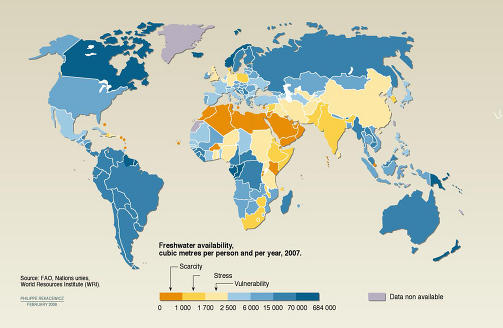
\includegraphics[width = 6cm]{picture/WaterScarcityMap.jpg}
  \end{wrapfigure}
  which make it a region where water is moderately overloaded. In our consideration, level 2, will provide more abundant behavior in a dynamical model(will it become water scarce or water sufficient in the future?). Thus we pick up China as our research object. To make our model more predictable and more reality connected.

  In order to explain why and how water is scarce in China,firstly,we state the water resources and water scarcity.Then We will give social and environmental reasons to water scarcity.

\subsection{Water resources}
China��s water resources are geographically divided into nine major river basins, including Yangtze, Yellow (Huang), Hai-Luan, Huai, Song-Liao, Pearl, Southeast, Southwest, and Northwest.The average volume of internal renewable water resources is estimated to be approximately 2812 billion $m^3$ per year,which ranks fifth in the world.\cite{Review}This volume includes both surface water and groundwater.

Approximately,98\% of China's surface water is recharged by precipitation.\cite{MWR2004a} average precipitation decreases in a spatial gradient from more than 2000 mm at the southeastern coastline to less than 200 mm at the northwestern hinterlands.\cite{MWR2004a}

\subsection{Physical scarcity}
Physical water scarcity is attributed to the shortfall in water resource volume to meet water needs.

We conclude physical water scarcity into 5 aspects as follow:
\begin{itemize}
\item Water shortages.

In normal water years, among 662 cities, 300 will have insufficient water supplies and 110 will experience severe water shortages; 30 out of 32 metropolitan areas with populations of more than 1 million people struggle to meet water demands.\cite{Li2006}The total annual water shortage is estimated to be 30-40 billion $m^3$ and is even larger in dry years.\cite{MWR2007b}

\item Water resource use and overexploitation.

North China has experienced heavy demand for water, and groundwater is an important source for water supply in this area.The average rate of water resource use ranged from 31.0\% to 91.7\% for basins in the north compared to rates of 1.7�C19.5\% in the south.\cite{MWR2007a}

\item Reduced instream flow and degraded aquatic ecosystems.

The discharge from the river to the ocean dwindled from an annual average of 24 billion $m^3$ in the 1950s to 1 billion $m^3$ in 2001.\cite{Xia2007}

\item Groundwater depletion.

It's recorded that groundwater depletion has increased in North China over the last two decades.Since the beginning of the 1980s,regions that overexploit groundwater have increased from 56 to 164 and the total area subject to groundwater overexploitation has increased from 87,000 $km^2$ to 180,000 $km^2$.\cite{MWR2007b}

\item Seawater intrusion and ground subsidence.

Seawater intrusion has occurred in 72 locations in Hebei, Shandong, and Liaoning provinces, covering a total area of 142 $km^2$ in 1992.\cite{WB2001}Cities such as Beijing, Tianjin, and Shanghai have been subject to ground subsidences of up to several meters.\cite{Shalizi2006}
\end{itemize}

\subsection{Economic water scarcity}
Economic water scarcity is caused by poor water quality that does not support any economic use of water rather than insufficient quantity.

We conclude economic water scarcity into two aspects as follow:
\begin{itemize}
\item Degrading water quality.

China��s general water quality trend is characterized by extended water sections of poor quality.In North China, all major river basins experience water quality degradation, and the percentage of monitored water sections ranked poor ranges from 50\% in the Yellow River basin to 78\% in the Hai River basin.\cite{SEPA}

China��s lakes and reservoirs are experiencing accelerated eutrophication and degraded water quality.

\item Socio-economic impact.

Degraded water quality has caused serious impacts on society. With a lack of clean, usable water, households, industries, and agriculture were forced to cut back their water use.In 2003, economic losses attributed to poor water quality were at least 158 billion yuan or 1.16\% of China��s annual GDP.\cite{WB2007a}

The cancer mortality rates associate with poor water quality.The rates of stomach, liver, and bladder cancers are highest in rural areas and the mortality rates of liver and stomach cancers in China are well above the world averages.\cite{WB2007a}
\end{itemize}

\subsection{Causes of water scarcity}
There are many factors contribute to China's water scarcity.We can classify them into social factors and environmental factors.

\paragraph{Social drivers:}As for the social factors,we can consider the relationship between population and water scarcity,water resource management.\cite{Review}List seven social reasons as follow:

\begin{enumerate}[\textbf{Factor} 1]
\item Rapid industrialization and urbanization associated with a large population
\item Fragmented institutional system of water resource management
\item Supply-driven water resources management and inefficient water use
\item Underdeveloped water rights system
\item Inadequate water pricing
\item Insufficient investment in environmental protection and weak pollution control
\item Policies not well integrated with each other
\end{enumerate}

\paragraph{Environmental drivers:}As for the environmental factors,we can consider natural conditions,climate,distribution of water resource.\cite{Review}List three factors as follow:

\begin{enumerate}[\textbf{Factor} 1]
\setcounter{enumi}{7}
\item The spatial distribution of China��s water resources is inconsistent with the local socioeconomic needs for water. The majority of China��s water resources are located in the southern part of the country, whereas the greatest need for water comes from northern and eastern China.
\item Climate change aggravates the problems.
\item The loss of glaciers and wetlands upstream decreases river runoffs.
\end{enumerate}


\section{China's water scarcity: Further Investigation and Prediction}

  For further investigation, we study with the data from National Bureau of Statistics of the People's Republic China\cite{ChinaDataBase}.According to our models, we should predetermine the alternative prominent parameters and grab all the data and try to analyses them and they relation.
  \subsection{Prominent variables' tendency}
  Using proper assumption and the past data in databases. We can using fitness method to determine the time dependency of our alternative parameters.
  In our consideration, following factors especially eye-catching.
  \begin{table}[!h]
  \centering
  \begin{tabular}{c|c}
  \hline
  $P$ & Population \\
  \hline
  $\text{PCGDP}$ & Per Capita Gross Domestic Product \\
  \hline
  $\text{IA}$ & Irrigation Area \\
  \hline
  $\text{ISP}$ & Iron and Steel Production \\
  \hline
  $\text{ElP}$ & Electricity Production. \\
  \hline
  $\text{EnC}$ & Engel's Coefficient \\
  \hline
  \end{tabular}
  \end{table}
  For further convenience, we will investigate their relation towards time at first.
    \paragraph{Population}
      The population growth model is various, for best concern, we use Logistic Model as the Population evolution model thus we can use the solution--Standard logistic sigmoid function as our target function by adding three basic coefficients.
      $$
      P(t) = \frac{K^P}{1+\exp[-\lambda^P(t-t_0^P)]}
      $$

    \paragraph{Per Capita Gross Domestic Product}
      As the largest developing country over the world, China has pretty high PCGDP growth rate. It seems like an exponential growth However, according to our data browse, some developed countries have already reach some obstacles. Thus we think it will be suitable if we apply Logistic model in the fitness model of $\text{PCGDP}$.
      $$
      \text{PCGDP}(t) = \frac{K^\text{PCGDP}}{1+\exp[-\lambda^\text{PCGDP}(t-t_0^\text{PCGDP})]}
      $$

    \paragraph{Irrigation Area}
      According to our observation, there is a strong evidence about linear growth of Irrigation Area. Consider the complicity and the fact we are just required to predict about 15 years, a polynomial fitting with power 2 is sufficient.
    $$
    \text{IA}(t) = A_0^\text{IA}+A_1^\text{IA} t + A_2^\text{IA} t^2
    $$

    \paragraph{Iron and Steel Production}
      The data of ISP perform in a similar way of IA, therefore we can use the same method to predict the ISP evolution.
    $$
    \text{ISP}(t) = A_0^\text{ISP}+A_1^\text{ISP} t + A_2^\text{ISP} t^2
    $$

    \paragraph{Electricity Production}
      The behavior of ELP is every bit as same as two parameters above, thus we just apply the same evolution equation form.
    $$
    \text{ELP}(t) = A_0^\text{ELP}+A_1^\text{ELP} t + A_2^\text{ELP} t^2
    $$

    \paragraph{Engel's Coefficient}
      Engel's Coefficient perform in a much different way. When it comes to the Engel, it make sense that with the development of society. It will keep decreasing as it used to be with a limit target: zero. Therefore we introduce a inverse proportion function to describe it's tendency.
    $$
    \begin{cases}
    \text{Enc}_\text{urban}(t) = C^\text{urban}/(t-t_0^\text{urban}) \\
    \text{Enc}_\text{rural}(t) = C^\text{rural}/(t-t_0^\text{rural})
    \end{cases}
    $$


    \begin{figure}[!h]
    \begin{center}
    \subfigure[$p(t)$]{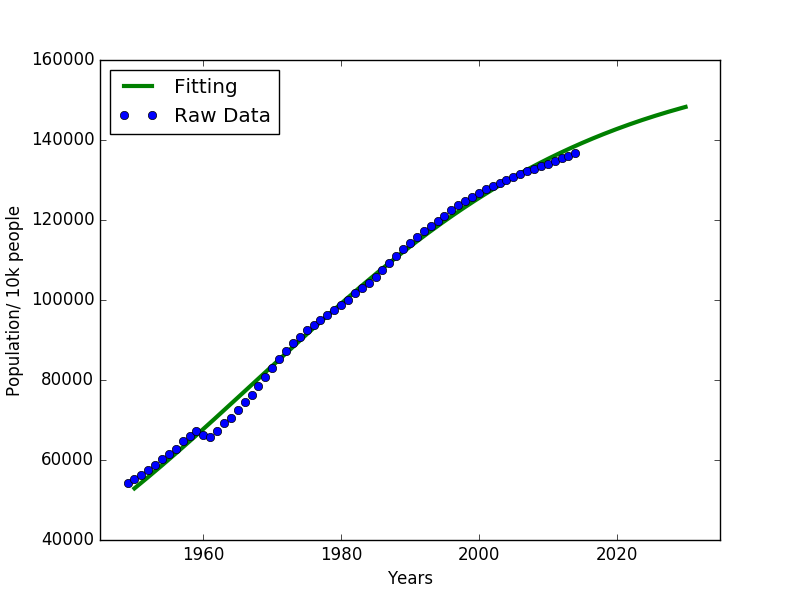
\includegraphics[width = 0.45\textwidth]{picture/Population.png}}
    \subfigure[$\text{PCGDP}(t)$]{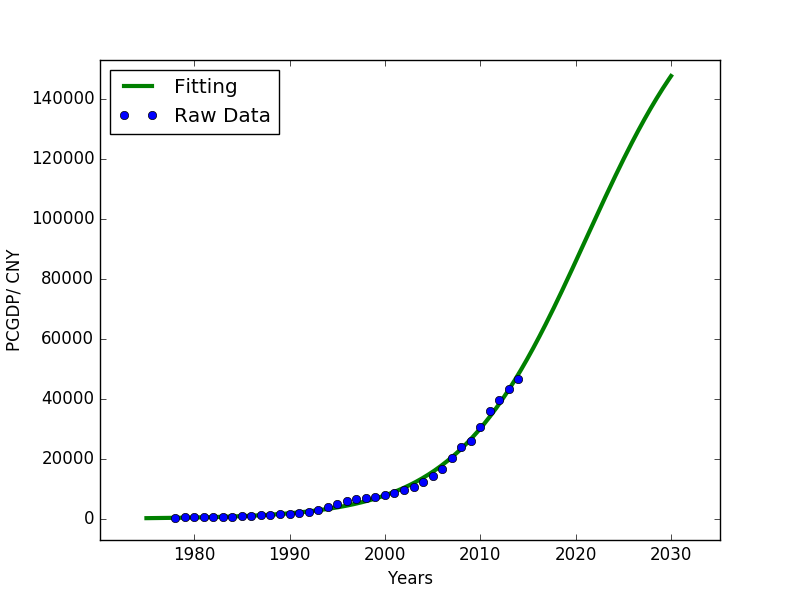
\includegraphics[width = 0.45\textwidth]{picture/PCGDP.png}}\\
    \subfigure[$\text{IA}(t)$]{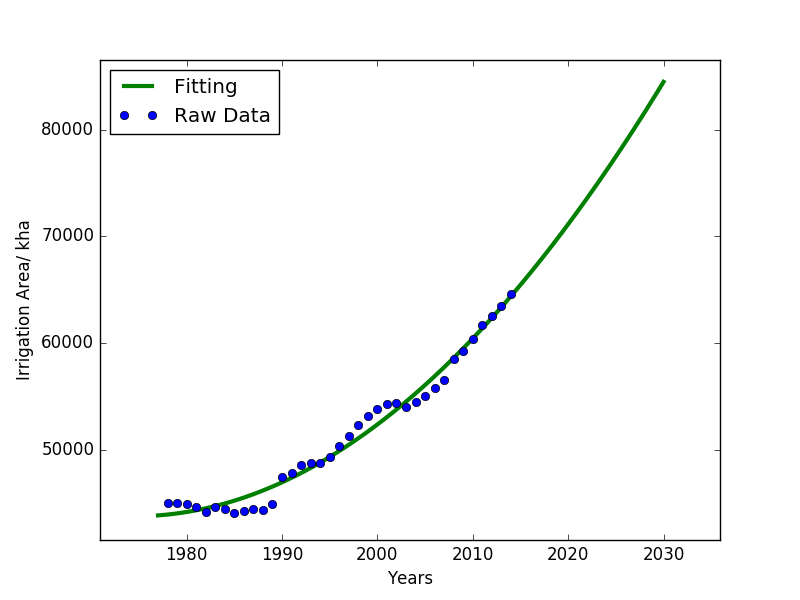
\includegraphics[width = 0.45\textwidth]{picture/IrrigationArea.png}}
    \subfigure[$\text{ISP}(t)$]{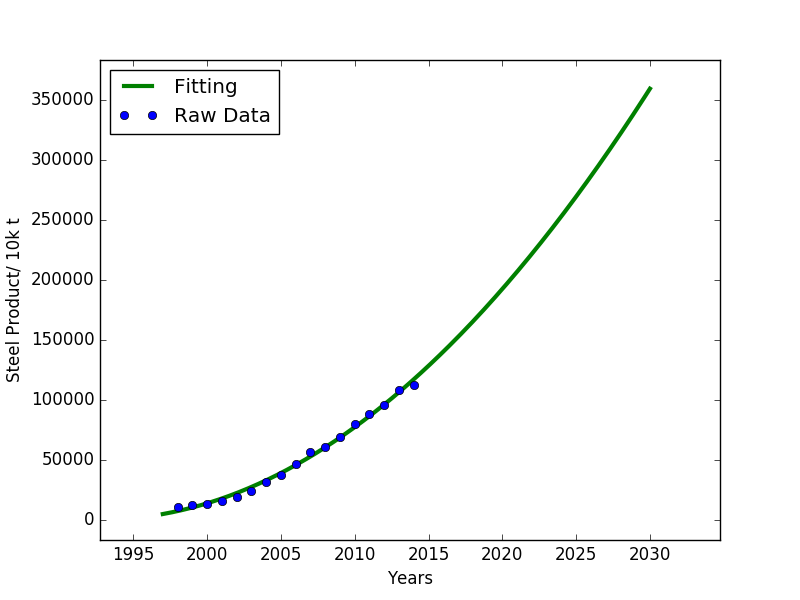
\includegraphics[width = 0.45\textwidth]{picture/SteelProduct.png}}\\
    \subfigure[$\text{ELP}(t)$]{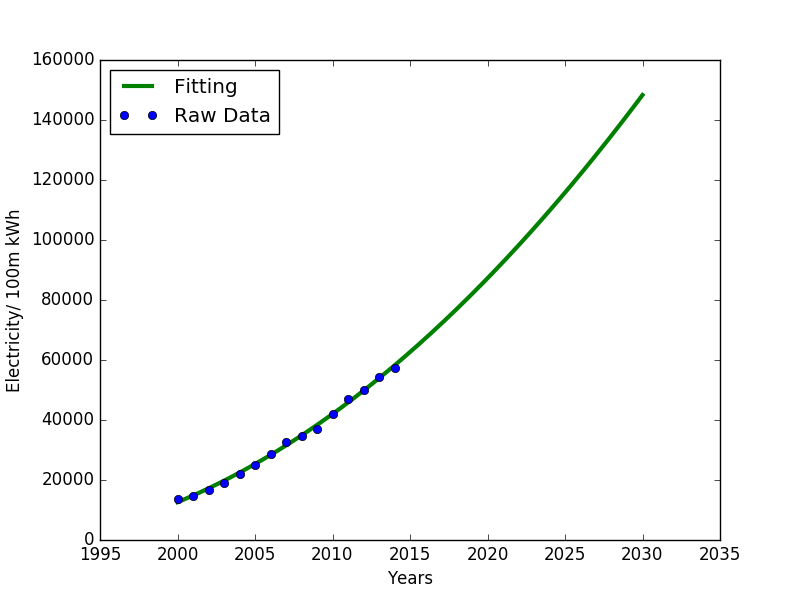
\includegraphics[width = 0.45\textwidth]{picture/Electricity.png}}
    \subfigure[$\text{Enc}(t)$]{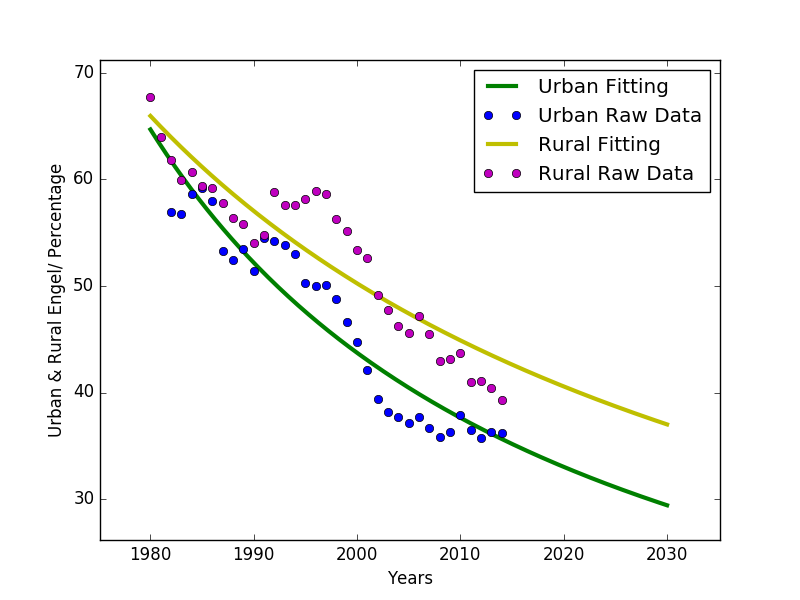
\includegraphics[width = 0.45\textwidth]{picture/Engel.png}}
    \end{center}
    \caption{Parameters fit: blue dots means the existed data which we refer from the national database, green lines stand for the optimized curve and the prediction value in the future }
    \label{fig: parameters fit}
    \end{figure}

    With the fitness method, we can get all the evolution of alternative prominent parameters in Figure~\ref{fig: parameters fit}, and the parameters in evolution equations in Tabl~\ref{tab: evolution par}:
    \begin{table}[!h]
      \centering
      \begin{tabular}{|l|l|}
      \hline
      $\left[t_0^P, \lambda^P,K^P\right]$ & [1968.14, 3.94\%, 161162.404] \\
      \hline
      $\left[t_0^\text{PCGDP}, \lambda^\text{PCGDP},K^\text{PCGDP}\right]$ & [2021.12, 14.9\%, 187060.984] \\
      \hline
      $\left[A_0^\text{IA},A_1^\text{IA},A_2^\text{IA}\right]$ & [5.155e+07, -5.217e+04, 13.21] \\
      \hline
      $\left[A_0^\text{ISP},A_1^\text{ISP},A_2^\text{ISP}\right]$ & [1.027e+09, -1.031e+06, 258.6] \\
      \hline
      $\left[A_0^\text{ELP},A_1^\text{ELP},A_2^\text{ELP}\right]$ & [3.125e+08, -3.146e+05, 79.19] \\
      \hline
      $\left[C^\text{urban},t_0^\text{urban},C^\text{rural},t_0^\text{rural}\right]$ & [1938.24, 2700.15, 1916.02, 4218.31] \\
      \hline
      \end{tabular}
      \caption{evolution parameters}
      \label{tab: evolution par}
    \end{table}


  \subsection{Relation between prominent parameters and variables}
    To investigate the relation between prominent parameters and variables, we firstly introduce the conception of  correlation. In statistics, dependence is any statistical relationship between two random variables or two sets of data, and correlation refers to any of a broad class of statistical relationships involving dependence.


    \paragraph{Pearson product-moment correlation coefficient}\cite{Pearson} is a measure of the linear correlation between two variables $X, Y$. If there is two datasets $\{x_1,x_2,\dots, x_n\}$ and $\{y_1,y_2,\dots, y_n\}$, then the formula for r is\cite{pearsonr}:
    $$
    r = \frac{\sum{(x_i-\bar{x})(y_i-\bar{y})}}{\sqrt{\sum{(x_i-\bar{x})^2}}\sqrt{\sum{(y_i-\bar{y})^2}}}
    $$

    \paragraph{Spearman's rank correlation coefficient} is a nonparametric measure of statistical dependence between two variables. It assesses how well the relationship between two variables can be described using a monotonic function. If there are no repeated data values, a perfect Spearman correlation of $+1$ or $-1$ occurs when each of the variables is a perfect monotone function of the other\cite{Spearman}\cite{spearmanr}. The Spearman correlation coefficient is defined as the Pearson correlation coefficient between the ranked variables\cite{rankedvariable}. For a sample of size n, the n raw scores $X_i,Y_i$ are converted ranks $x_i, y_i$, and $\rho$ is computed from:
    $$
    \rho = 1 - \frac{6\sum{(x_i-y_i)^2}}{n(n^2-1)}
    $$

    \paragraph{Kendall rank correlation coefficient} is a statistic used to measure the association between two measured quantities. Let $(x_1, y_1),(x_2, y_2),\dots,(x_n, y_n)$ be a set of observations of the joint random variables $X$ and $Y$ respectively, such that all the values of $(x_i)$ and $(y_i)$ are unique. Any pair of observations $(x_i,y_i)$ and $(x_j, y_j)$, where $i\neq j$, are said to be concordant if the ranks for both elements agree: that is, if both $x_i > x_j$ and $y_i > y_j$ or if both $x_i < x_j$ and $y_i < y_j$. They are said to be discordant, if $x_i > x_j$ and $y_i < y_j$ or if $x_i < x_j$ and $y_i > y_j$. If $x_i = x_j$ or $y_i = y_j$, the pair is neither concordant nor discordant. Thus the $\tau$ coefficient is defined as\cite{Kendall}\cite{kendalltau}:
    $$
    \tau = \frac{(\text{number of concordant pairs}) - (\text{number of discordant pairs})}{\frac{1}{2} n (n-1)}
    $$

    Using coefficients above, we get a map about the relation between prominent parameters and consumption variables.

    \begin{table}[!htb]

      \centering
      \begin{tabular}{l||c|c|c|c}
      \hline
      Data                & Pearson $(r_p,p)$                        & Spearman $(r_s,p)$       & Kendall $(\tau, p)$ & Average \\
      \hline

      $\text{IWC}\sim P$ & (0.669,0.0245)                   &(0.627,0.0388)   &(0.455,0.0516)     &   0.584\\
      \hline
      $\text{IWC}\sim \text{PCGDP}$ &(0.614,0.0444)         &(0.627,0.0388)   &(0.455,0.0516)     &   0.565\\
      \hline
      $\text{IWC}\sim \text{ELP}$ &(0.648,0.0311)           &(0.627,0.0388)   &(0.455,0.0516)     &   0.577\\
      \hline
      $\text{IWC}\sim \text{ISP}$ &(0.653,0.0294)           &(0.627,0.0388)   &(0.455,0.0516)     &   0.577\\
      \hline\hline
      $\text{AWC}\sim P$ &(0.924,4.95e-5)                   &(0.927,3.97e-5)  &(0.782,0.000815)     &   0.878\\
      \hline
      $\text{AWC}\sim \text{PCGDP}$ &(0.936,2.28e-5)        &(0.927,3.97e-5)  &(0.782,0.000815)     &   0.882\\
      \hline
      $\text{AWC}\sim \text{IA}$ &(0.927,4.10e-5)           &(0.927,3.97e-5)  &(0.782,0.000815)     &  0.879 \\
      \hline\hline
      $\text{DWC}\sim P$ &(0.844,0.00108)                   &(0.836,0.00133)  &(0.745,0.00141)     &   0.808\\
      \hline
      $\text{DWC}\sim \text{PCGDP}$ &(0.806,0.00276)        &(0.836,0.00133)  &(0.745,0.00141)     &   0.796\\
      \hline
      $\text{DWC}\sim \text{Enc}_\text{urban}$ &(-0.785,0.00417) &(-0.809,0.00256) &(-0.600,0.0102)     &  -0.731 \\
      \hline
      $\text{DWC}\sim \text{Enc}_\text{rural}$ &(-0.419,0.199)   &(-0.315,0.345)   &(-0.204,0.383)     &   -0.313\\
      \hline

      \end{tabular}
      \caption{Coefficients: Coefficients of correlation in different standard}
      \label{tab: coefficients}
    \end{table}



  \subsection{Fitness method in consumption variables}
  To investigate the evolution of consumption variables, We first investigate the correlation between one specific consumption with one specific prominent parameters.

  \paragraph{Industry Water Consumption}
  According to coefficients calculation result in Table~\ref{tab: coefficients}, taking all $P, \text{PCGDP}, \text{ELP}, \text{ISP}$ in to account will be rational. Moreover, The correlation between IWC and those factors are kinda weird, therefore using polynomial fit is unreasonable here. Further more, once we find that the IWC will never be negative and the shape or past data, it will be convenient for us to using Gaussian function here. At least we get the result in Table~\ref{tab:IWC - parameters} and Figure~\ref{fig: IWC para}.

  \begin{table}[!h]
  \centering
  \begin{tabular}{l||c|c|c}
  \hline
  Parameters & $p_0$  &  $p_1$  & $p_2$ \\ \hline
  $P$       &  1.43e3 & 7.62e-9 & 1.34e5 \\ \hline
  $\text{PCGDP}$ & 1.45e3 &  3.35e-10 & 3.31e4 \\ \hline
  $\text{ELP}$   & 1.44e3  &  3.10e-10 & 4.45e4 \\ \hline
  $\text{ISP}$   & 1.44e3  &  5.50e-11 & 8.40e4 \\ \hline
  \end{tabular}
  \caption{IWC - parameters: $p_0\exp{[-p_1 (\text{para}-p_2)^2]}$}
  \label{tab:IWC - parameters}
  \end{table}

  \begin{figure}[!h]
  \centering
  \subfigure[$P$]{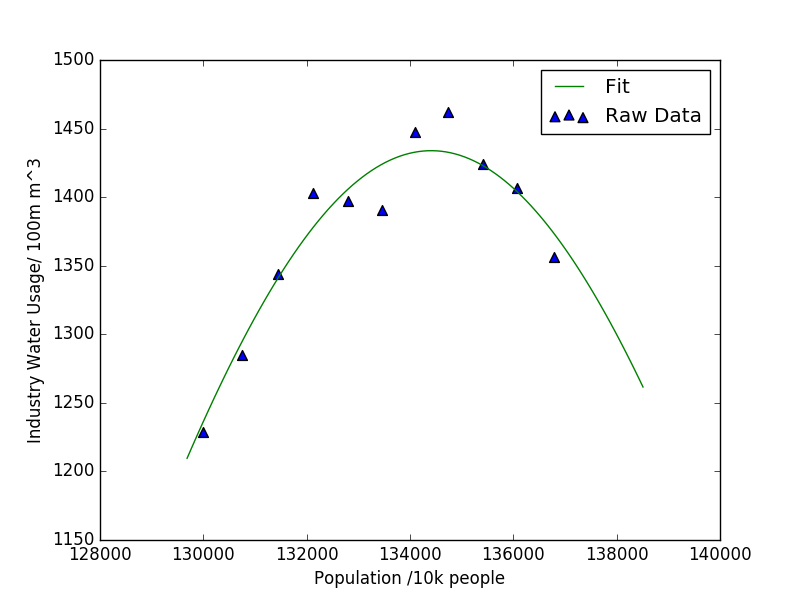
\includegraphics[width = 0.45\textwidth]{picture/Population-Industry.png}}
  \subfigure[$\text{PCGDP}$]{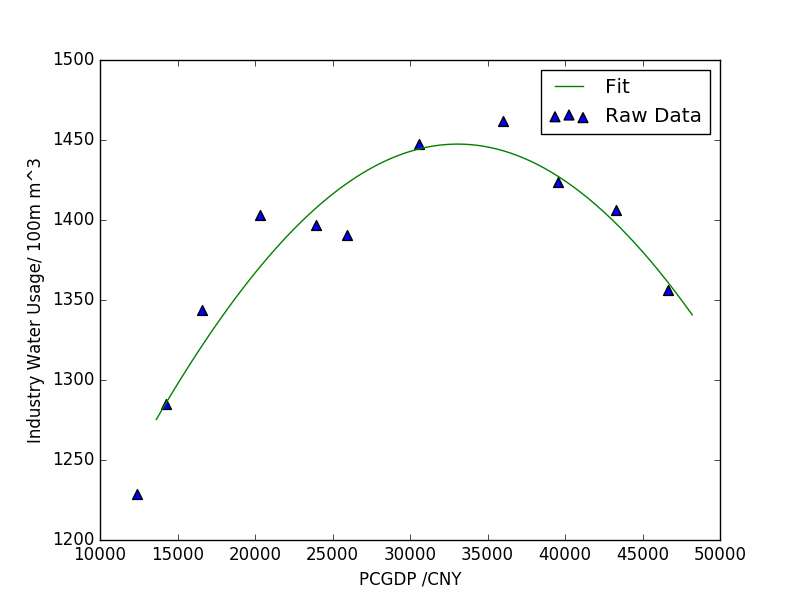
\includegraphics[width = 0.45\textwidth]{picture/PCGDP-Industry.png}}
  \subfigure[$\text{ELP}$]{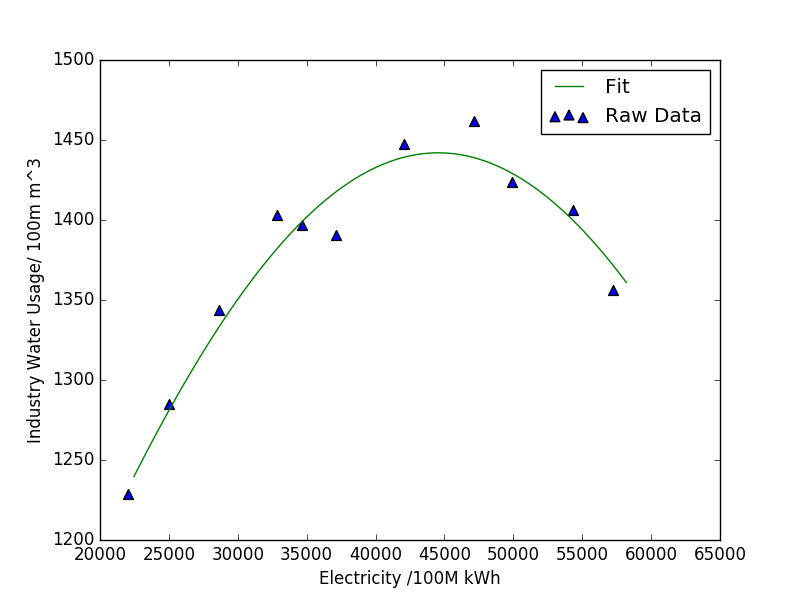
\includegraphics[width = 0.45\textwidth]{picture/Electricity-Industry.png}}
  \subfigure[$\text{ISP}$]{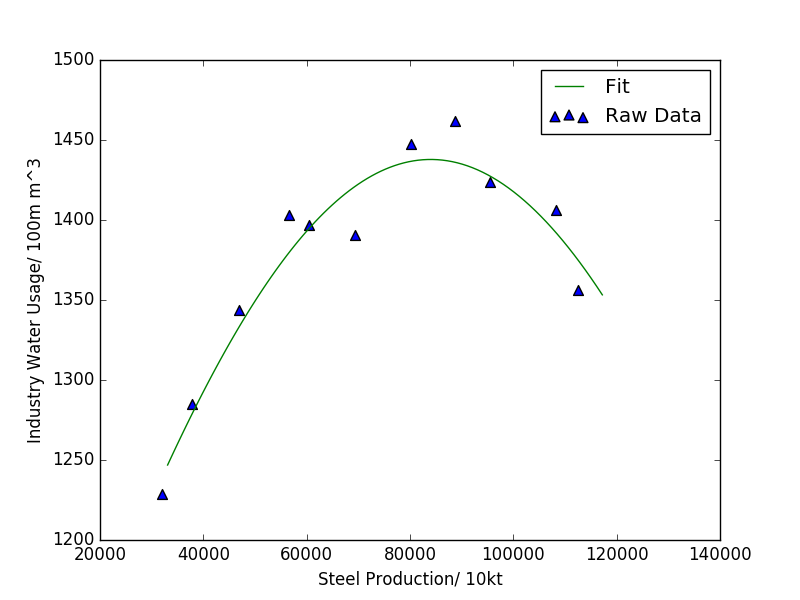
\includegraphics[width = 0.45\textwidth]{picture/SteelProduct-Industry.png}}
  \caption{IWC - parameters}
  \label{fig: IWC para}
  \end{figure}


  \paragraph{Agricultural Water Consumption}
  According to coefficients calculation result in Table~\ref{tab: coefficients}, taking all $P, \text{PCGDP}, \text{IA}$in to account will be reasonable. Due to to fact that we have no clue about the form of their relation, using polynomial fitting will be a proper choice. The results are in Table~\ref{tab:AWC - parameters} and Figure~\ref{fig: AWC para}

  \begin{table}[!h]
  \centering
  \begin{tabular}{l||c|c|c}
  \hline
  Parameters & $p_0$  &  $p_1$  & $p_2$ \\ \hline
  $P$       &  -1.31e3 & 5.07e-2 & 3.42e4 \\ \hline
  $\text{PCGDP}$ & -1.50e3 &  9.54e-3 & -5.18e5 \\ \hline
  $\text{IA}$   & -1.09e3  &  3.20e-2 & -9.09e4 \\ \hline
  \end{tabular}
  \caption{AWC - parameters: $p_0 +p_1 (\text{para}-p_2)$ }
  \label{tab:AWC - parameters}
  \end{table}

  \begin{figure}[!h]
  \centering
  \subfigure[$P$]{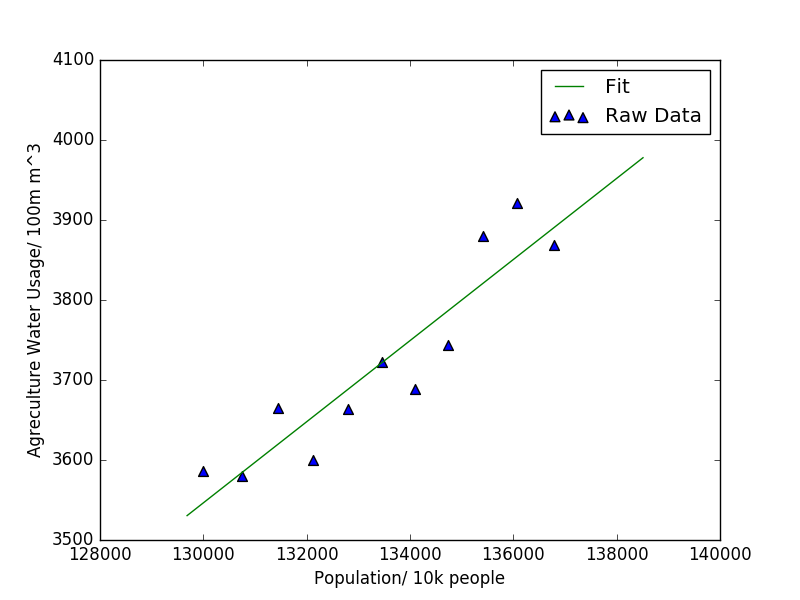
\includegraphics[width = 0.3\textwidth]{picture/Population-Agreculture.png}}
  \subfigure[$\text{PCGDP}$]{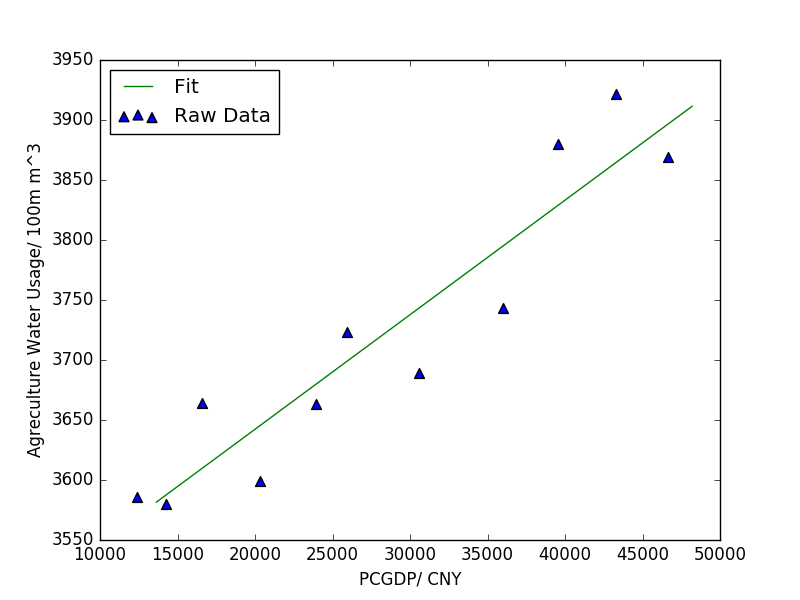
\includegraphics[width = 0.3\textwidth]{picture/PCGDP-Agreculture.png}}
  \subfigure[$\text{IA}$]{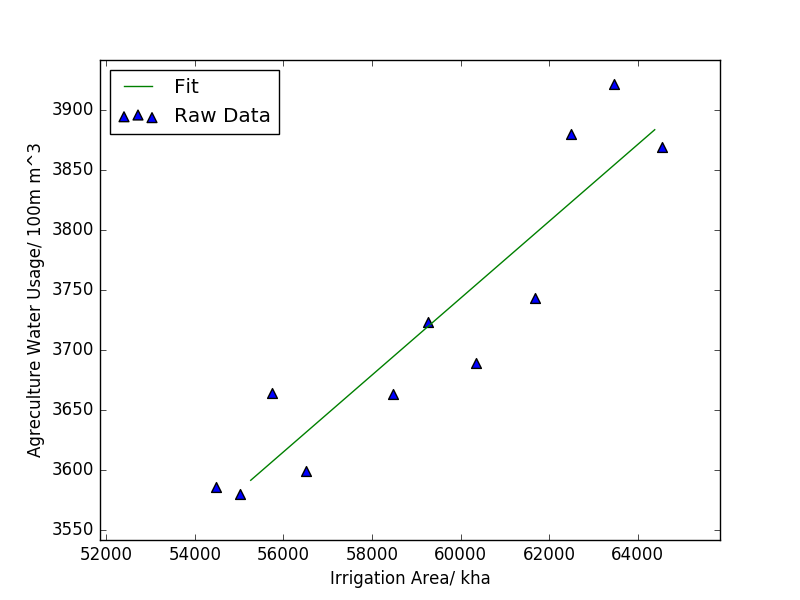
\includegraphics[width = 0.3\textwidth]{picture/IrrigationArea-Agreculture.png}}
  \caption{AWC - parameters}
  \label{fig: AWC para}
  \end{figure}

  \paragraph{Domestic Water Consumption}
  The data about DWC and other parameters is kinda weird. Firstly, according to the coefficient in Table~\ref{tab: coefficients}. We think the Engel's Coefficients is kinda useless and it will be reasonable to eliminate them from right now. Moreover, make the whole fit system more general, this time we try exponential fit, and the result are showed in Table~\ref{tab:DWC - parameters} and Figure~\ref{fig: DWC para}.

  \begin{table}[!h]
  \centering
  \begin{tabular}{l||c|c|c}
  \hline
  Parameters & $p_0$  &  $p_1$  & $p_2$ \\ \hline
  $P$       &  3.95e2 & -2.16e-5 & 1.05e5 \\ \hline
  $\text{PCGDP}$ & 3.98e2 &  -3.82e-6 & -1.30e5 \\ \hline
  \end{tabular}
  \caption{DWC - parameters: $p_0\exp{[-p_1 (\text{para}-p_2)]}$}
  \label{tab:DWC - parameters}
  \end{table}

  \begin{figure}[!h]
  \centering
  \subfigure[$P$]{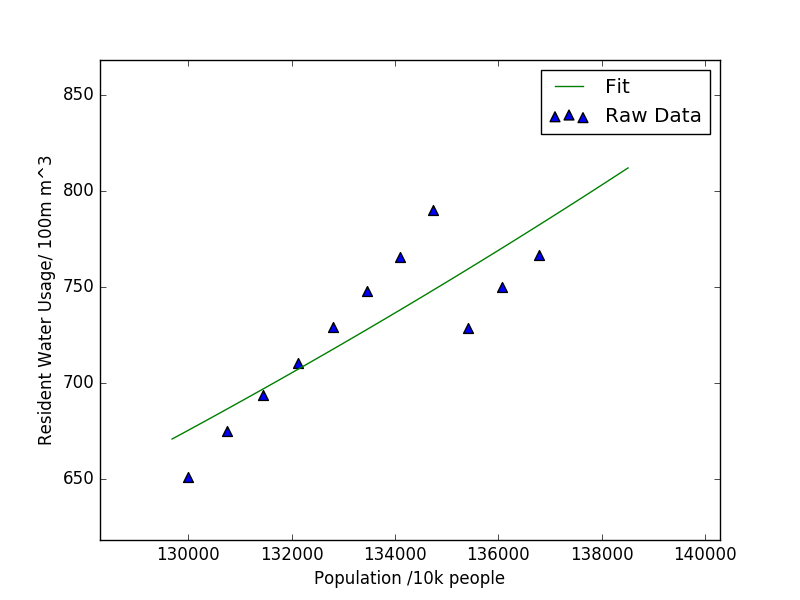
\includegraphics[width = 0.45\textwidth]{picture/Population-Resident.png}}
  \subfigure[$\text{PCGDP}$]{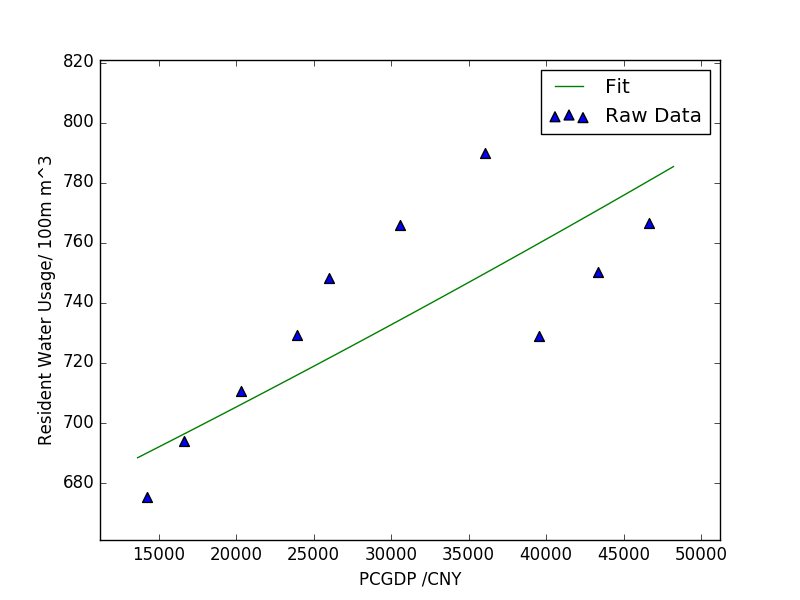
\includegraphics[width = 0.45\textwidth]{picture/PCGDP-Resident.png}}
  \caption{DWC - parameters}
  \label{fig: DWC para}
  \end{figure}

  \subsection{Prediction of future water supply ability}
  With the discussion above, now it's time to predict the future water supply ability $A$. Firstly, we introduce intermediate variables to separate the Water Consumption variables into several parts. For instance, $\text{DWC} = \text{DWC}(P,\text{PCGDP})$, with the investigation above, we can write in a separated form:
  $$
  \text{DWC}(t) =\text{DWC}(P(t),\text{PCGDP}(t)) = \frac{\alpha_{P}\text{DWC}(P)+\alpha_{\text{PCGDP}}\text{DWC}(\text{PCGDP})}{\alpha_{P}+\alpha_{PCGDP}}
  $$
  Where $\alpha_P$ and $\alpha_\text{PCGDP}$ stand for the average correlation coefficients of $P,\text{PCGDP}$ to $\text{DWC}.$
  And the form of variables like $\text{DWC}(P)$ or $\text{DWC}(\text{PCGDP})$ are exactly the correlation we got int Table~\ref{tab:IWC - parameters} -~\ref{tab:DWC - parameters}.
  Others consumption variables are exactly same as this example. The analysis result are shown in Figure~\ref{fig: consumption predict}.

  \begin{figure}[!h]
  \subfigure[IWC]{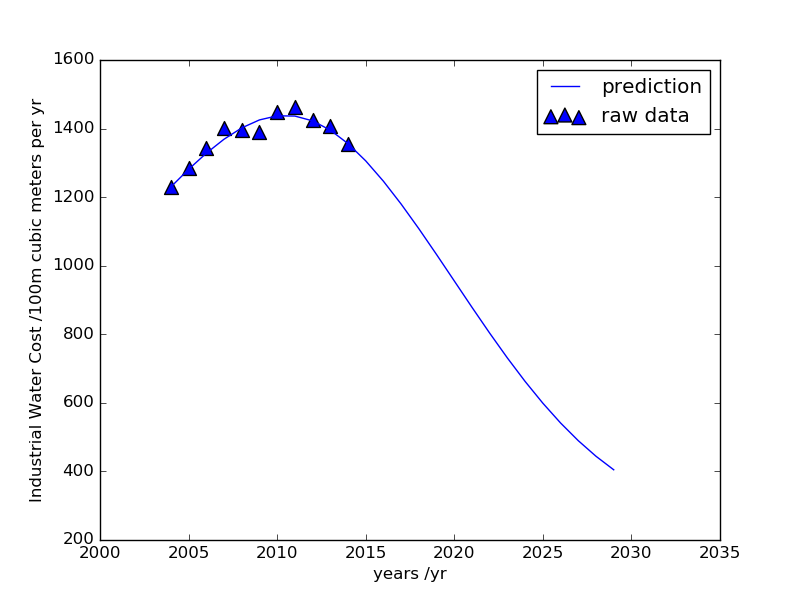
\includegraphics[width = 0.32\textwidth]{picture/Indust-pre.png}}
  \subfigure[AWC]{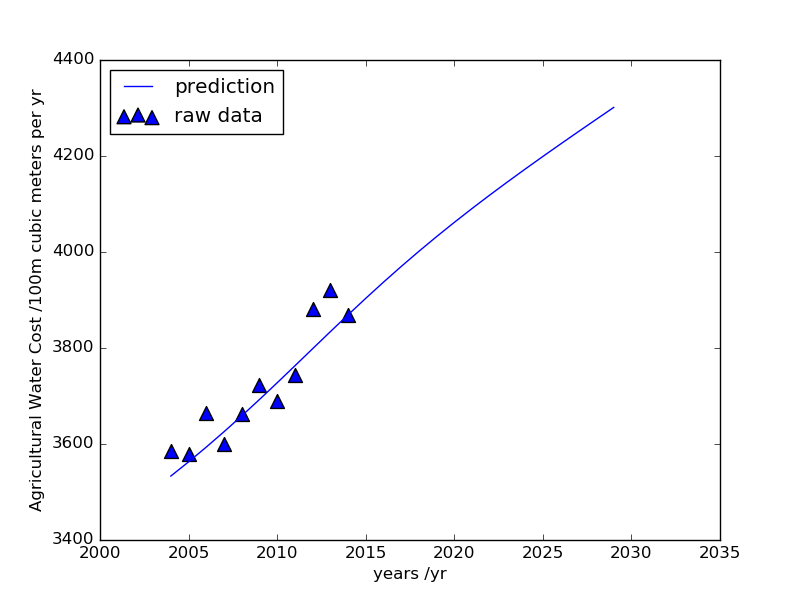
\includegraphics[width = 0.32\textwidth]{picture/Agri-pre.png}}
  \subfigure[DMC]{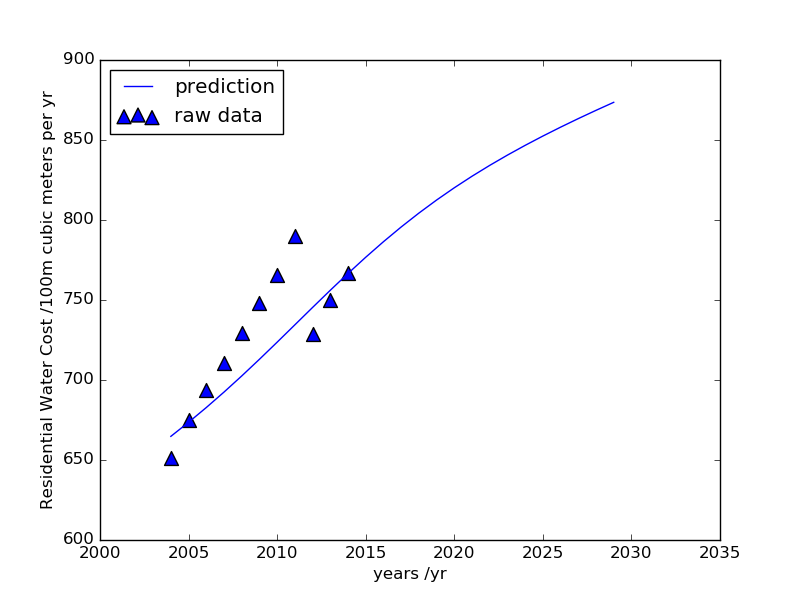
\includegraphics[width = 0.32\textwidth]{picture/Resident-pre.png}}
  \caption{consumption predict}
  \label{fig: consumption predict}
  \end{figure}

  With the prediction value of water consumption, we can easily get the water supply ability through Equation~\ref{equ: Ability}. And the result is showed in Figure~\ref{fig: supply ability} and in Table~\ref{tab: supply ability}.


  \begin{figure}[!h]
  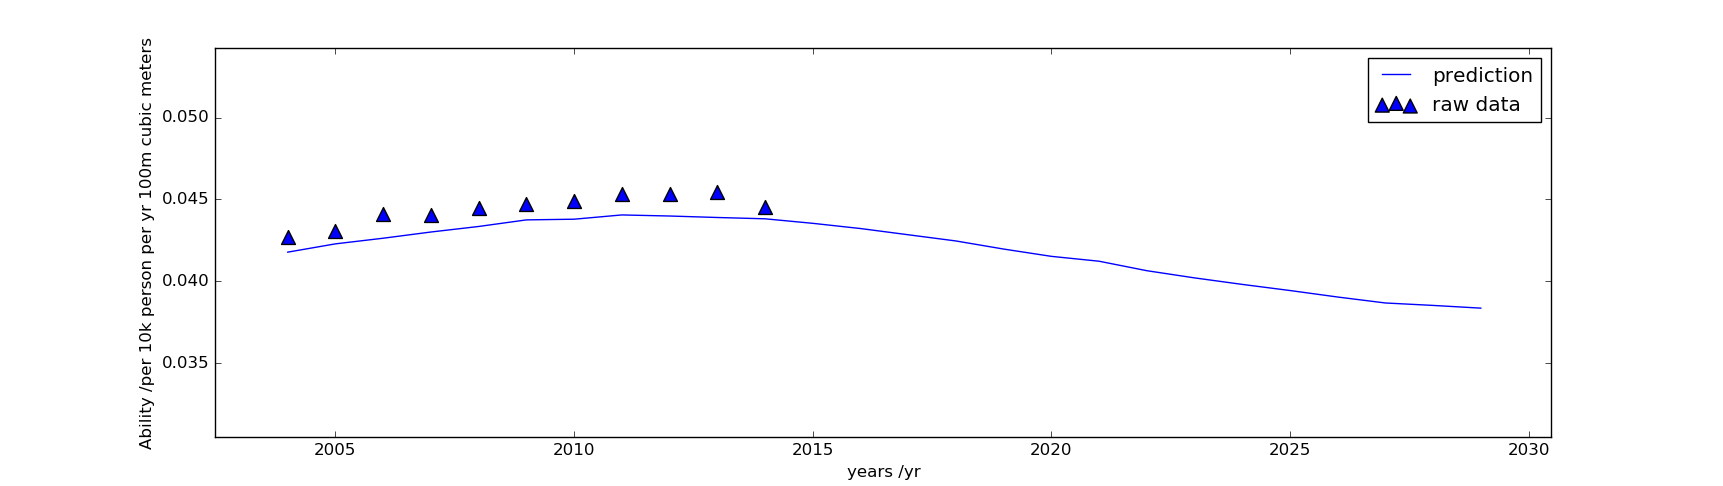
\includegraphics[width = 0.9\textwidth]{picture/Ability-pre.png}
  \caption{Water supply ability prediction}
  \label{fig: supply ability}
  \end{figure}
  \begin{table}[!h]
  \centering
  \begin{tabular}{|l ||c|c|c|c|c|c|c|c|}
  \hline
  year & 2014 & 2015 & 2016 & 2017 & 2018 & 2019 & 2020& 2021 \\ \hline
  A/$\text{m}^3$ & 437.61 &436.00 &433.80 &429.60 & 423.19 & 419.65 &414.43 & 410.93 \\ \hline \hline
  year & 2022 & 2023 & 2024 & 2025 & 2026 & 2027 & 2028& 2029 \\ \hline
  A/$\text{m}^3$ & 407.03 & 400.66 & 397.18 &393.60 & 389.96 & 388.18 & 385.10 & 383.17 \\ \hline
  \end{tabular}
  \caption{Water supply ability prediction: A is Annual water supplies per person}
  \label{tab: supply ability}
  \end{table}

  According to our prediction, the water scarcity in China is going to be more and more severe if there is no intervention plan. And actually we are about the turning point of annual water supply per person drop. There will be about 12.4\% drop in the following 15 years. So proper intervention plan should be undertaken to prevent this scarcity.

\section{Intervention plan designing and prediction}
  As shown in our prediction. China will suffer from water scarcity in 15 years. Therefore we designed an intervention plan to avoid this situation.
  \subsection{Population Intervention}
  The huge population base has become the most serious problem in China and plays a leading role in China's water stress problem. To improve the ability of water supply family planning can play a significant role. We decrease the population growth rate to 1\% and the result is obvious.The ability increases by 10.0 $\text{m}^3 \text{per person}$ up to 2030. The result is showed in Figure~\ref{fig: Population control}.
  \begin{figure}[!h]
  \centering
  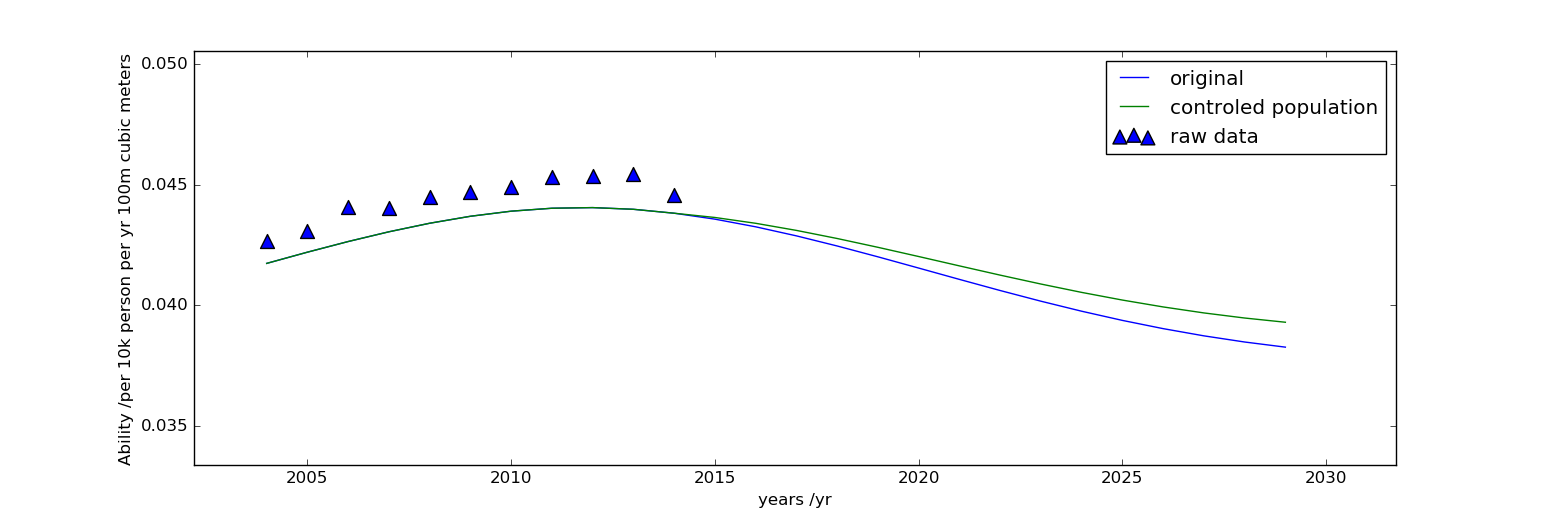
\includegraphics[width = 0.9\textwidth]{picture/popcontrol.png}
  \caption{Population control}
  \label{fig: Population control}
  \end{figure}


  \subsection{Water Distribution Intervention}
  One of the most important issue in China's water allocation problem is the uneven distributed water resources. By developing infrastructure, a better water allocation will be possible to achieve. This will, for example, benefit out irrigation in remote areas. With increasing irrigation area by 30\%, the ability will increase about 20.0 $\text{m}^3 \text{per person}$ up to 2030 according to our model. The result in showed in Figure~\ref{fig: Irrigation are increase}.

  \begin{figure}[!h]
  \centering
  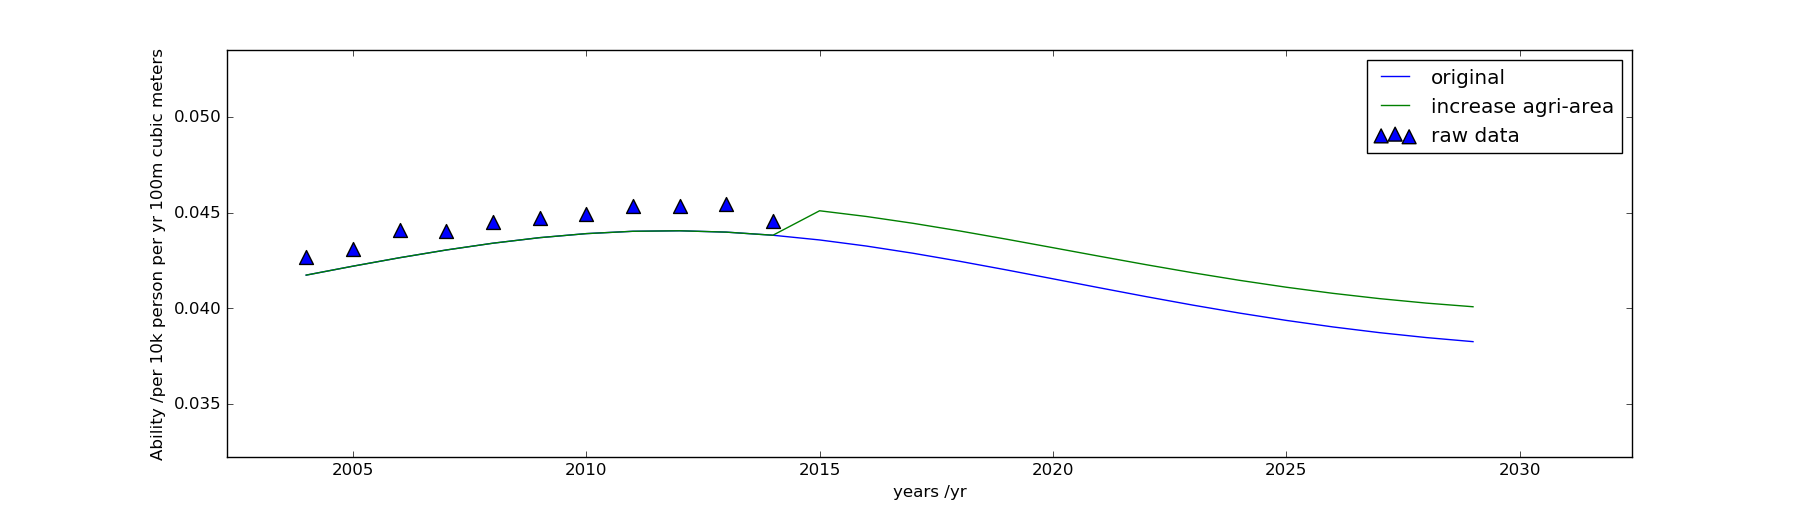
\includegraphics[width = 0.9\textwidth]{picture/icrarea.png}
  \caption{Irrigation Area Increase}
  \label{fig: Irrigation are increase}
  \end{figure}

  \subsection{Industrial Intervention}
  Virtual water has been a hot topic recently, which refers to the hidden flow of water if food or other commodities are traded from one place to another. In our model, the water-consuming industry is evaluated by iron and steel production plus electricity. Therefore water stress can be alleviated through reducing iron and steel production and import more steel, which is a considerable amount of virtual water. The result of reducing 30\% of the steel production is shown in Figure~\ref{fig: Iron and Steel Production decrease}, the ability increases by 9.0 $\text{m}^3 \text{per person}$.
  \begin{figure}[!h]
  \centering
  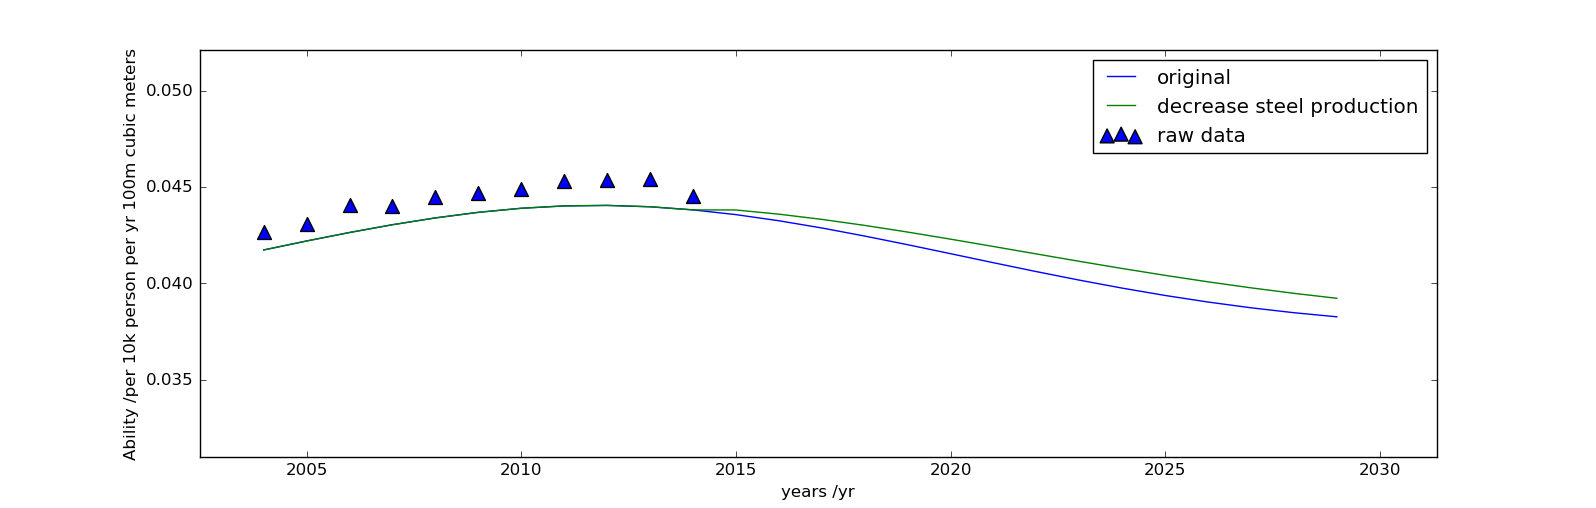
\includegraphics[width = 0.9\textwidth]{picture/drssteel.png}
  \caption{fig: Iron and Steel Production decrease}
  \label{fig: Iron and Steel Production decrease}
  \end{figure}

  \subsection{Overview}
  By simultaneously implementing our intervention plans, the ability of China increases by approximately 40.0 $\text{m}^3 \text{per person}$ up to 2030, as is shown in. It's result is showed in Figure~\ref{fig: overview intervention}
  \begin{figure}[!h]
  \centering
  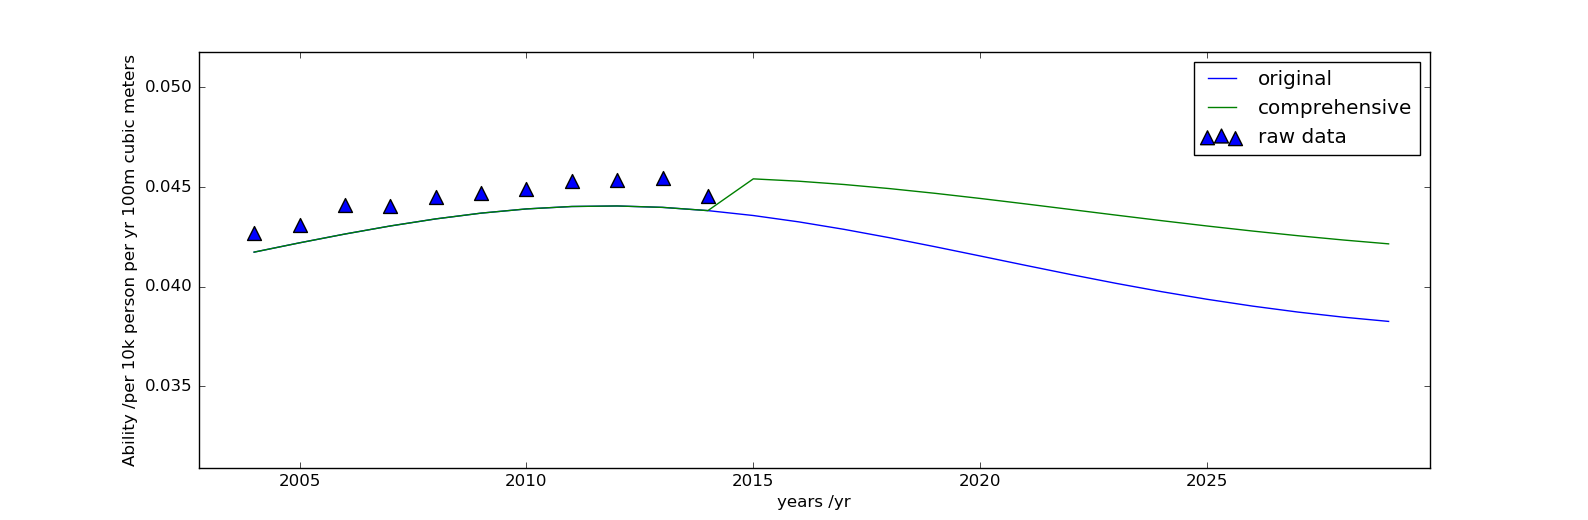
\includegraphics[width = 0.9\textwidth]{picture/comprehensive.png}
  \caption{Overview intervention}
  \label{fig: overview intervention}
  \end{figure}

  \subsection{Climate and uncertainty evaluation}
  In history, water scarcity also occurs when the climate changes. However, the probability of a drought which have the ability to affect the whole region is pretty low. To estimate climate's effects and other uncertain issues, normal distributed random variables is added to every prominent parameters with corresponding variances which is fitted from raw data. The variance of Ability shows the sensitivity of a given region.
  The sensitivity of a given region can be reduced by constructing infrastructure such as reservoirs and dams. As is shown in Figure~\ref{fig: constructing infrastructures} the ability curve become more steady after constructing infrastructures.
  \begin{figure}[!h]
  \centering
  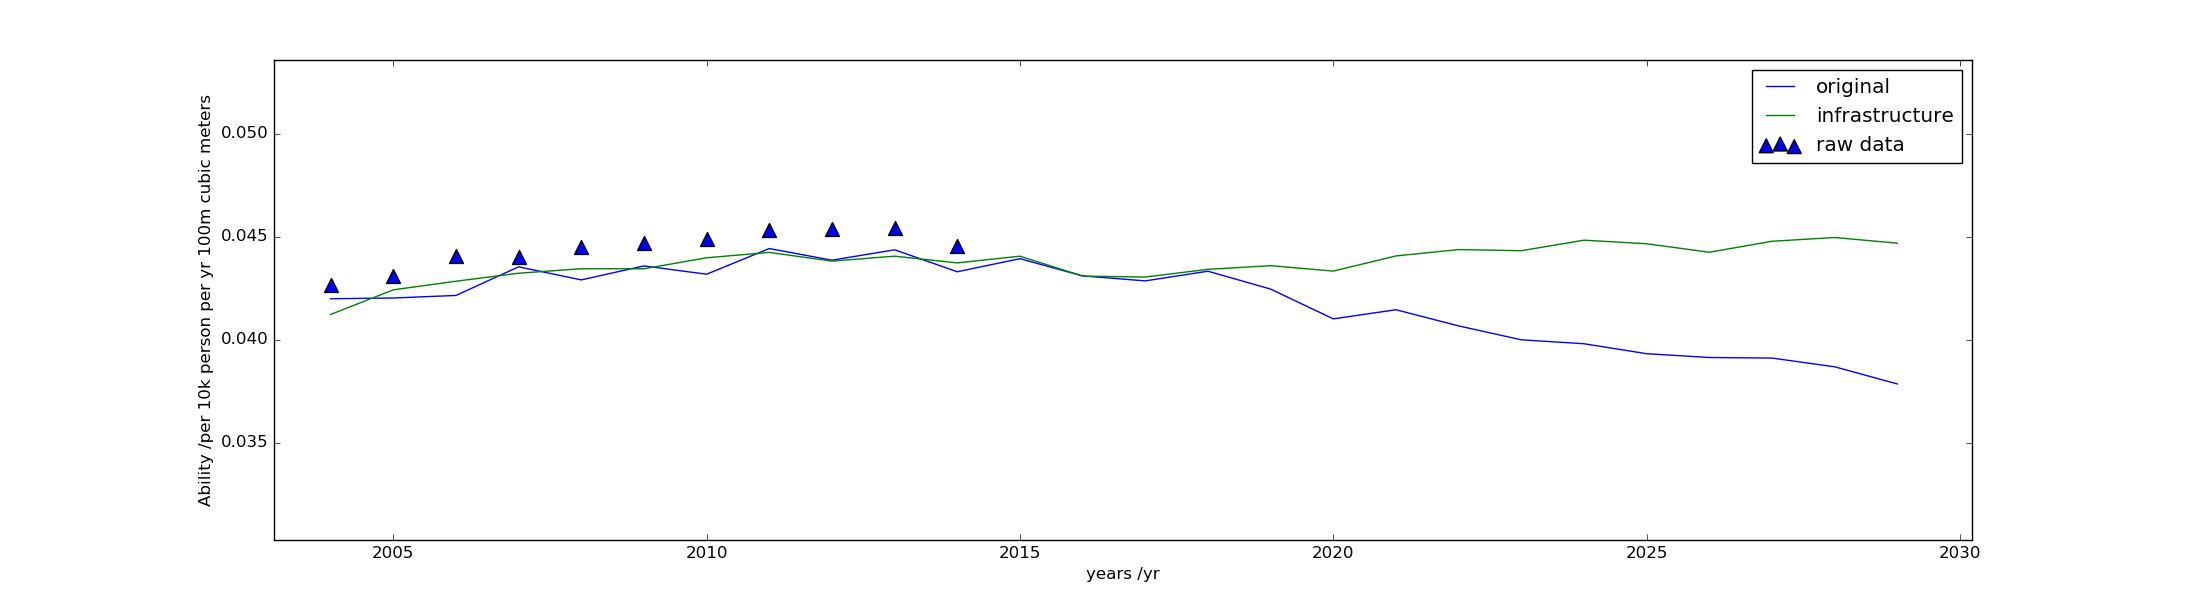
\includegraphics[width = 0.9\textwidth]{picture/sense.png}
  \caption{Constructing infrastructures}
  \label{fig: constructing infrastructures}
  \end{figure}

\section{Executive Summary}

  \subsection{Approach to the problem}
  Firstly, we decide to focus on industrial, agricultural and domestic water consumption which can effectively represent the water supply ability. Secondly, we try to find the relationship between each part of water consumption and other prominent parameters that can represent the state of society (such as population, PCGDP ...) from the data provided by National Bureau of Statistics of the PRC. Thirdly, we can use the tendency of those prominent parameters to predict the evolution of water consumption therefore decide the water supply ability. Finally, we introduce the intervention plan through altering the model's corresponding parameters and structures.

  \subsection{Conclusion}
  According to our research, we come to the following conclusion.

  \begin{itemize}
    \item The annual water supply per capita is a practical and widely accepted standard for water scarcity evaluation.
    \item China is country suffering from water scarcity. The main reasons are: uneven spatial distribution of water resources, rapid growing population and consequent issues and poor water resource management.
    \item According to our model, China's water scarcity will become even more severe (the annual water supply per capita will decrease by 12.4\%) in the future if no intervention plan is undertaken.
    \item Taking the internal mechanism into consideration, we introduce 3 possible intervention plans for the situation of China: Population control, Water distribution intervention, Industrial intervention. And the annual water supply per capita will increase by 10.0, 20.0, 9.0 $\text{m}^3 \text{per person}$ respectively.
    \item With the stochastic behavior of climate is taken into account, the construction of hydrological infrastructures can reduce the risk of water scarcity under natural disasters such as drought and flood.
    \item The above prediction under the stochastic behavior also shows that our model is stable under reasonable parameters' fluctuation.
  \end{itemize}

  \subsection{Strengths and Weaknesses}
    \paragraph{Strengths}
    \begin{itemize}
      \item We maximized the utility of raw statistic data, so the model have a strong reliability.
      \item In spite of being a totally statistical model, we use the statistic data to find the internal dynamics among the consumption variables and the prominent parameters, which works pretty good according to past data.
      \item Our model has a great flexibility, new factors of water consumption can be added into our model easily.
    \end{itemize}

    \paragraph{Weaknesses}
    \begin{itemize}
      \item For the simplicity, we ignore the internal structure of China's water distribution which may also be important in our problem.
      \item Due to the heavy dependency on raw data, the prediction time range of our model is limited.
    \end{itemize}


\begin{thebibliography}{99}
  \bibitem{wikiwaterscarcity} https://en.wikipedia.org/wiki/Water\_scarcity
  \bibitem{research1} Water Scarcity. International Decade for Action \'Water for Life\' 2005�C2015. un.org. Retrieved 20 October 2013.
  \bibitem{research2}  \"Water Stress\". Retrieved 20 October 2013.
  \bibitem{research3} \"Water Scarcity. Threats\". WWF. 2013. Retrieved 20 October 2013.

  \bibitem{AbilityMeasure} {Falkenmark and Lindh 1976, quoted in UNEP/WMO.Climate Change 2001: Working Group II: Impacts,Adaptation and Vulnerability. UNEP. Retrieved 3 February 2009.}
  \bibitem{WaterCycle} trinityrivertexas.org, Living with the Trinity Lesson Plan 1: The Natural Water Cycle and the Urban Water Cycle
  \bibitem{WaterScarcityMap} http://www.unep.org/dewa/vitalwater
  \bibitem{Review} China's water scarcity,Yong Jiang,Journal of Environmental Management Volume 90, Issue 11, August 2009, Pages 3185�C3196
  \bibitem{MWR2004a} Ministry of Water Resources, Beijing, China (2004) http://www.mwr.gov.cn/english1/20040802/38161.asp retrieved in July 2007
  \bibitem{Li2006} http://news.xinhuanet.com/environment/2006-09/13/content\_5084123.htm (2006) accessed July 2007
  \bibitem{MWR2007b}MWR (Ministry of Water Resources, P.R. China) The 11th Five-Year Plan of National Water Resources Development, Gazette of the Ministry of Water Resources of the P.R China, 2007 (2007), pp. 34�C48
  \bibitem{MWR2007a}MWR (Ministry of Water Resources, P.R. China)Water Resources Bulletin 2006 Ministry of Water Resources, Beijing, China (2007)
  \bibitem{Xia2007}J. Xia L. Zhang, C.M. Liu, J.J. Yu Towards better water security in North China Water Resource Management, 21 (2007), pp. 233�C247
  \bibitem{MWR2007b} MWR (Ministry of Water Resources, P.R. China)The 11th Five-Year Plan of National Water Resources Development, Gazette of the Ministry of Water Resources of the P.R China, 2007 (2007), pp. 34�C48
  \bibitem{WB2001} WB (World Bank)Agenda for Water Sector Strategy for North China: Summary Report World Bank, Washington DC, USA (2001)
  \bibitem{Shalizi2006} Z. Shalizi Addressing China's Growing Water Shortages and Associated Social and Environmental Consequences World Bank, Washington D.C., USA (2006)
  \bibitem{SEPA} SEPA (State Environmental Protection Administration, P.R. China)China Environmental Bulletins 1990�C2006 State Environmental Protection Administration, Beijing, China (1991�C2007)
  \bibitem{WB2007a}WB (World Bank) Cost of Pollution in China: Economic Estimates of Physical Damages World Bank, Washington DC, USA (2007)

  \bibitem{ChinaDataBase} http://www.stats.gov.cn
  \bibitem{Pearson} https://en.wikipedia.org/wiki/Pearson\_product-moment\_correlation\_coefficient\#Definition
  \bibitem{pearsonr} http://www.statsoft.com/textbook/glosp.html\#Pearson\%20Correlation
  \bibitem{Spearman} https://en.wikipedia.org/wiki/Spearman\%27s\_rank\_correlation\_coefficient
  \bibitem{spearmanr} Zwillinger, D. and Kokoska, S. (2000). CRC Standard Probability and Statistics Tables and Formulae. Chapman \& Hall: New York. 2000. Section 14.7
  \bibitem{rankedvariable} Myers, Jerome L.; Well, Arnold D. (2003). Research Design and Statistical Analysis (2nd ed.). Lawrence Erlbaum. p. 508
  \bibitem{Kendall} https://en.wikipedia.org/wiki/Kendall\_rank\_correlation\_coefficient
  \bibitem{kendalltau} W.R. Knight, ��A Computer Method for Calculating Kendall��s Tau with Ungrouped Data��, Journal of the American Statistical Association, Vol. 61, No. 314, Part 1, pp. 436-439, 1966

\end{thebibliography}


%==========================================================

\begin{comment}
%===============================appendices===============================
    \begin{appendices}
    %\renewcommand{\thesection}{\Alph{chapter}.}

      \section{First appendix}

    some text...


Here are simulation programmes we used in our model as follow.\\


\textbf{\textcolor[rgb]{0.98,0.00,0.00}{Input matlab source:}}
\lstinputlisting[language=Matlab]{./code/matlab1.m}


      \section{Second appendix}

    some more text\textcolor[rgb]{0.98,0.00,0.00}{\textbf{Input C++ source:}}
\lstinputlisting[language=C++]{./code/sudoku.cpp}

    \end{appendices}

\end{comment}